% =====================================================================
%  SLIDE CHIẾU — BÁO CÁO TIẾN ĐỘ DỰ ÁN CONTAGION
%  Biên dịch:  xelatex baocao_slides.tex   (XeLaTeX vì có tiếng Việt)
%  Đây là bản để CHIẾU. Lời nói đầy đủ nằm ở file baocao_noidung.pdf
% =====================================================================
\documentclass[aspectratio=169,11pt]{beamer}

\usepackage{fontspec}
\setmainfont{Times New Roman}
\usefonttheme{professionalfonts}
\usepackage{amsmath}
\usepackage{graphicx}

\usetheme{Madrid}
\usecolortheme{seahorse}
\setbeamertemplate{navigation symbols}{}
\setbeamertemplate{itemize items}[circle]
\setbeamerfont{frametitle}{size=\large}

\title[Contagion: lan truyền prompt injection]{Contagion: đo lan truyền prompt injection trong mạng LLM agent}
\subtitle{Báo cáo tiến độ}
\author[Người báo cáo]{Người báo cáo: \underline{\hspace{3.2cm}}}
\institute[Lớp/Đơn vị]{Lớp/Đơn vị: \underline{\hspace{4cm}}}
\date{\underline{\hspace{3.5cm}}}

\begin{document}

\begin{frame}
  \titlepage
\end{frame}

\begin{frame}{Tóm tắt trong một phút}
  \begin{itemize}
    \item \textbf{Đối tượng:} mạng nhiều LLM agent phối hợp (kiểu MetaGPT, AutoGen).
    \item \textbf{Câu hỏi:} một agent bị nhiễm $\Rightarrow$ lan được bao xa, và cái gì
          quyết định nó sống sót qua mỗi lần chuyển giao?
    \item \textbf{Cách làm:} khung đo với \textbf{hai protocol độc lập}, 5 model / 4 họ
          model, 3 topology.
    \item \textbf{Kết quả:} 4 phát hiện chính + 1 phát hiện của chính nhóm
          \textbf{đã bị rút lại} sau khi tìm ra lỗi thiết kế đo.
    \item \textbf{Hiện trạng:} bản thảo bài báo đã xong, đúng giới hạn \textbf{8 trang}.
  \end{itemize}
\end{frame}

\begin{frame}{Bối cảnh: vì sao đây là vấn đề mới}
  \begin{itemize}
    \item Mạng agent ghép bằng \textbf{văn bản tự do}: đầu ra agent này là đầu vào agent kia.
    \item Mỗi lần chuyển giao là một \textbf{ranh giới tin cậy}.
    \item \textbf{Prompt injection gián tiếp:} chỉ dẫn độc hại được nhúng vào nguồn dữ
          liệu agent đọc (tài liệu, kết quả công cụ, email).
    \item Đã biết: \emph{một} agent bị hijack được (InjecAgent, AgentDojo, Liu \& Gong
          2024); injection tồn tại dai dẳng trong một ứng dụng (Greshake 2023).
    \item \textbf{Chỗ trống:} chưa có khung đo trả lời ``đi được bao xa, chặn ở đâu''.
  \end{itemize}
\end{frame}

\begin{frame}{Bốn câu hỏi nghiên cứu}
  \begin{enumerate}
    \item \textbf{RQ1 --- Đo lường:} xác suất sống sót qua \emph{từng} lần chuyển giao,
          và nó phụ thuộc vào cái gì?
    \item \textbf{RQ2 --- Tính cộng dồn:} con số ``tỉ lệ tấn công thành công'' của
          benchmark một-agent có \emph{nhân lên} được thành dự đoán cho pipeline không?
    \item \textbf{RQ3 --- Tiêu chí an toàn:} ``chỉ số lây nhiễm $R_0<1$ thì an toàn'' có
          dùng được cho mạng agent không?
    \item \textbf{RQ4 --- Đánh giá phòng thủ:} làm sao biết một defense thật sự có tác
          dụng?
  \end{enumerate}
\end{frame}

\begin{frame}{Phương pháp (1): hai protocol độc lập}
  \begin{block}{Protocol A --- đo từng cạnh có kiểm soát}
    \emph{ép} đầu ra agent nguồn thành ``đã nhiễm'' $\to$ đưa cho agent nhận $\to$ chấm.
    Kết quả: $s_i=\Pr[C_i{=}1 \mid C_{i-1}{=}1]$.
  \end{block}
  \begin{block}{Protocol B --- chạy tự nhiên}
    Chạy cả mạng như bình thường $\to$ đo ASR đầu-cuối và chỉ số lây nhiễm $R_0$.
  \end{block}
  \begin{itemize}
    \item \textbf{Vì sao hai protocol?} Một cách đo thì không phân biệt được
          ``\emph{đo sai}'' với ``\emph{hiểu sai hệ thống}''.
    \item Chấm bằng công cụ \textbf{tất định}, \emph{không} dùng LLM làm giám khảo.
  \end{itemize}
\end{frame}

\begin{frame}{Phương pháp (2): cấu hình}
  \begin{itemize}
    \item Hai họ nhiệm vụ: \textbf{ngữ nghĩa} (Task A) và \textbf{marker}
          \texttt{BANANA-77} (Task B); nhiệm vụ độc hại phải \emph{cạnh tranh} với việc hợp lệ.
    \item \textbf{3 ngữ cảnh công việc hợp lệ} xoay vòng theo trial.
    \item \textbf{5 model / 4 họ:} Llama 3.3 70B · DeepSeek V3.2 · Claude Sonnet 4.5 ·
          Nova Pro · qwen2.5:7b (local, miễn phí).
    \item \textbf{3 topology:} chuỗi (chain) · hình sao (star fan-in) · hình cây (tree).
    \item Lưu \emph{toàn bộ đầu ra thô} $\Rightarrow$ chấm lại được mà không tốn thêm chi phí.
  \end{itemize}
\end{frame}

\begin{frame}{Kết quả 1: ``giả định Markov'' là một \emph{đẳng thức}}
  \begin{itemize}
    \item Trong chuỗi: $C_i{=}1 \Rightarrow C_{i-1}{=}1$
          $\Rightarrow \mathrm{ASR}=\prod_i s_i^{\mathrm{nat}}$
          \textbf{đúng bằng đại số}, không phải giả định.
    \item Kiểm bằng số đo thật (khớp tuyệt đối):
          chuỗi 4 agent $0{,}850=0{,}850$; chuỗi 7 agent $0{,}450=0{,}450$;
          sao $0{,}725$; cây $0{,}800$.
    \item \textbf{Câu hỏi thật:} con số đo \emph{cách ly} có bằng con số \emph{trong
          chuỗi thật}? $\to$ \textbf{transportability}.
    \item Đây là chỗ mọi benchmark một-agent đang \emph{ngầm giả định}, chưa ai kiểm.
  \end{itemize}
\end{frame}

\begin{frame}{Kết quả 2: giả định đó \emph{thất bại}, sai số lớn dần theo độ sâu}
  \begin{itemize}
    \item DeepSeek V3.2: tích cách ly khớp ASR tới $\mathbf{2{,}2\%}$ $\Rightarrow$ chuyển được.
    \item Llama 3.3 70B: cạnh giữa cách ly $0{,}233$ nhưng trong chuỗi $\mathbf{0{,}875}$
          $\Rightarrow$ \textbf{thấp hơn $3{,}75\times$}.
  \end{itemize}
  \begin{center}
  \small
  \begin{tabular}{|l|c|c|c|c|}
  \hline
  \textbf{Model} & \textbf{Chuỗi} & \textbf{Sai số} & \textbf{$\rho$} & \textbf{Dốc (\%/hop)}\\
  \hline
  qwen2.5:7b & n=7 & $31\%\to 89\%$ & $+1{,}00$ & $+11{,}8$\\
  Llama 3.3 70B & n=15 & $0\%\to 92\%$ & $+0{,}77$ & $+6{,}8$\\
  DeepSeek V3.2 & n=8 & $7\%$--$35\%$ & $-0{,}07$ & $+0{,}1$\\
  \hline
  \end{tabular}
  \end{center}
  \begin{itemize}
    \item $\Rightarrow$ \textbf{độ dốc của đường cong là phép chẩn đoán}: một chuỗi dài,
          một lần chạy, biết ngay model đó có cộng dồn được hay không.
  \end{itemize}
\end{frame}

\begin{frame}{Cơ chế: hình thức thông điệp quyết định --- chênh $\mathbf{14}$ lần}
  \begin{itemize}
    \item Cùng mục tiêu, cùng agent nhận, cùng cách chấm, cùng phân công:
  \end{itemize}
  \begin{center}
  \small
  \begin{tabular}{|l|c|}
  \hline
  \textbf{Cách trình bày thông điệp} & \textbf{Xác suất sống sót}\\
  \hline
  Một câu khẳng định trần & $0{,}067$\\
  Nhúng trong một sản phẩm công việc & $\mathbf{0{,}967}$\\
  \hline
  \end{tabular}
  \end{center}
  \begin{itemize}
    \item Giải thích kết quả 2: artefact ``chuẩn hoá'' dùng khi đo cách ly
          \emph{không đại diện} cho thông điệp thật.
    \item Tự kiểm tra lại: phát lại nội dung bắt được khớp \textbf{2/3} cạnh
          (cạnh 3: $0{,}733$ so với $0{,}947$) --- báo cáo đúng $2/3$.
  \end{itemize}
\end{frame}

\begin{frame}{Kết quả 3: tiêu chí ngưỡng dịch tễ \emph{vô hiệu} trên mạng feed-forward}
  \begin{itemize}
    \item \textbf{Định lý:} ma trận lây nhiễm của \emph{mọi} mạng không có vòng, sắp theo
          topology, là \textbf{tam giác chặt} $\Rightarrow$ mọi giá trị riêng bằng $0$
          $\Rightarrow \rho(M)=0$ \textbf{luôn luôn}, bất kể cạnh mạnh cỡ nào.
    \item Nghĩa là ``$R_0<1$ $\Rightarrow$ an toàn'' được thoả mãn \emph{tầm thường} ---
          không phân biệt được hệ an toàn với hệ nguy hiểm.
    \item Thực nghiệm:
      \begin{itemize}
        \item chuỗi 7 agent: $R_0=0{,}821<1$ nhưng ASR $=0{,}450$
        \item hình sao: $R_0=0{,}420<1$ nhưng ASR $=0{,}725$
      \end{itemize}
    \item \textbf{Độ lan tới} và \textbf{khả năng tái lây} là hai rủi ro khác nhau.
  \end{itemize}
\end{frame}

\begin{frame}{Kết quả 3 (tiếp): khi có vòng lặp, tiêu chí trở nên \emph{có} hiệu lực}
  \begin{itemize}
    \item Mô hình thật: manager giao việc cho 2 worker, worker \textbf{báo cáo ngược lại}.
    \item Tổng quát cho $w$ worker (kiểm bằng số tới $4{,}4{\times}10^{-16}$):
          $\rho(M)=\sqrt{\sum_j a_jc_j}$ với \emph{mọi} $w$.
          Không có báo cáo ngược ($c_j{=}0$) $\Rightarrow \rho=0$ bất kể cạnh mạnh cỡ nào.
    \item \textbf{Quy tắc thiết kế:} vượt ngưỡng $\iff \sum_j a_jc_j>1$;
          đối xứng thì $w\,s^2>1$: ở $s{=}0{,}5$ cần \textbf{5} worker, $0{,}7$ cần
          \textbf{3}, $0{,}9$ cần \textbf{2}.
    \item \textbf{Hai dự đoán ngược nhau} trên hai model đã đo:
  \end{itemize}
  \begin{center}
  \small
  \begin{tabular}{|l|c|c|l|}
  \hline
  \textbf{Model} & $\sum_j a_jc_j$ & $\rho$ & \textbf{Dự đoán $\to$ Kết quả}\\
  \hline
  Llama 3.3 70B & $1{,}800$ & $\mathbf{1{,}342}$ & vượt ngưỡng $\to$ \textbf{giữ nguyên} \checkmark\\
  qwen2.5:7b & $0{,}578$ & $0{,}760$ & dưới ngưỡng $\to$ \textbf{tắt dần} \checkmark\\
  \hline
  \end{tabular}
  \end{center}
  \begin{itemize}
    \item Llama: manager tái nhiễm $0{,}725$ $[0{,}572;0{,}839]$; vòng 5 manager
          $0{,}700$, worker $0{,}925$/$0{,}975$ $\Rightarrow$ \textbf{lưu cữu}.
    \item qwen: manager tái nhiễm $0{,}775$ $[0{,}625;0{,}877]$ $\to$ vòng 5 còn
          $0{,}650$; worker dừng ở $0{,}475$/$0{,}525$, \emph{không} bão hoà
          $\Rightarrow$ \textbf{yếu dần}.
    \item Giới hạn: mới 5 vòng --- đủ phân biệt ``yếu dần'' với ``bão hoà'',
          \emph{chưa} đủ chứng minh tắt hẳn.
  \end{itemize}
\end{frame}

\begin{frame}{Kết quả 4: đánh giá phòng thủ cần ``chỗ để giảm'' (hiệu ứng sàn)}
  \begin{itemize}
    \item Cùng defense, cùng kiểu tấn công, cùng code chấm điểm:
      \begin{itemize}
        \item Claude: không phòng thủ $0{,}10 \to$ redaction $0{,}00$
              $\Rightarrow$ ``trông hoàn hảo'' nhưng chỉ có $10\%$ để bảo vệ.
        \item DeepSeek: $1{,}00 \to 0{,}00$ $\Rightarrow$ defense làm hết việc.
      \end{itemize}
    \item \textbf{Kết luận:} thiếu baseline ``không phòng thủ'' thì \emph{không xác định
          được} hiệu quả của defense.
    \item Biến hình tấn công (tách chuỗi, chèn khoảng trắng) phá được redaction.
  \end{itemize}
  \begin{center}
    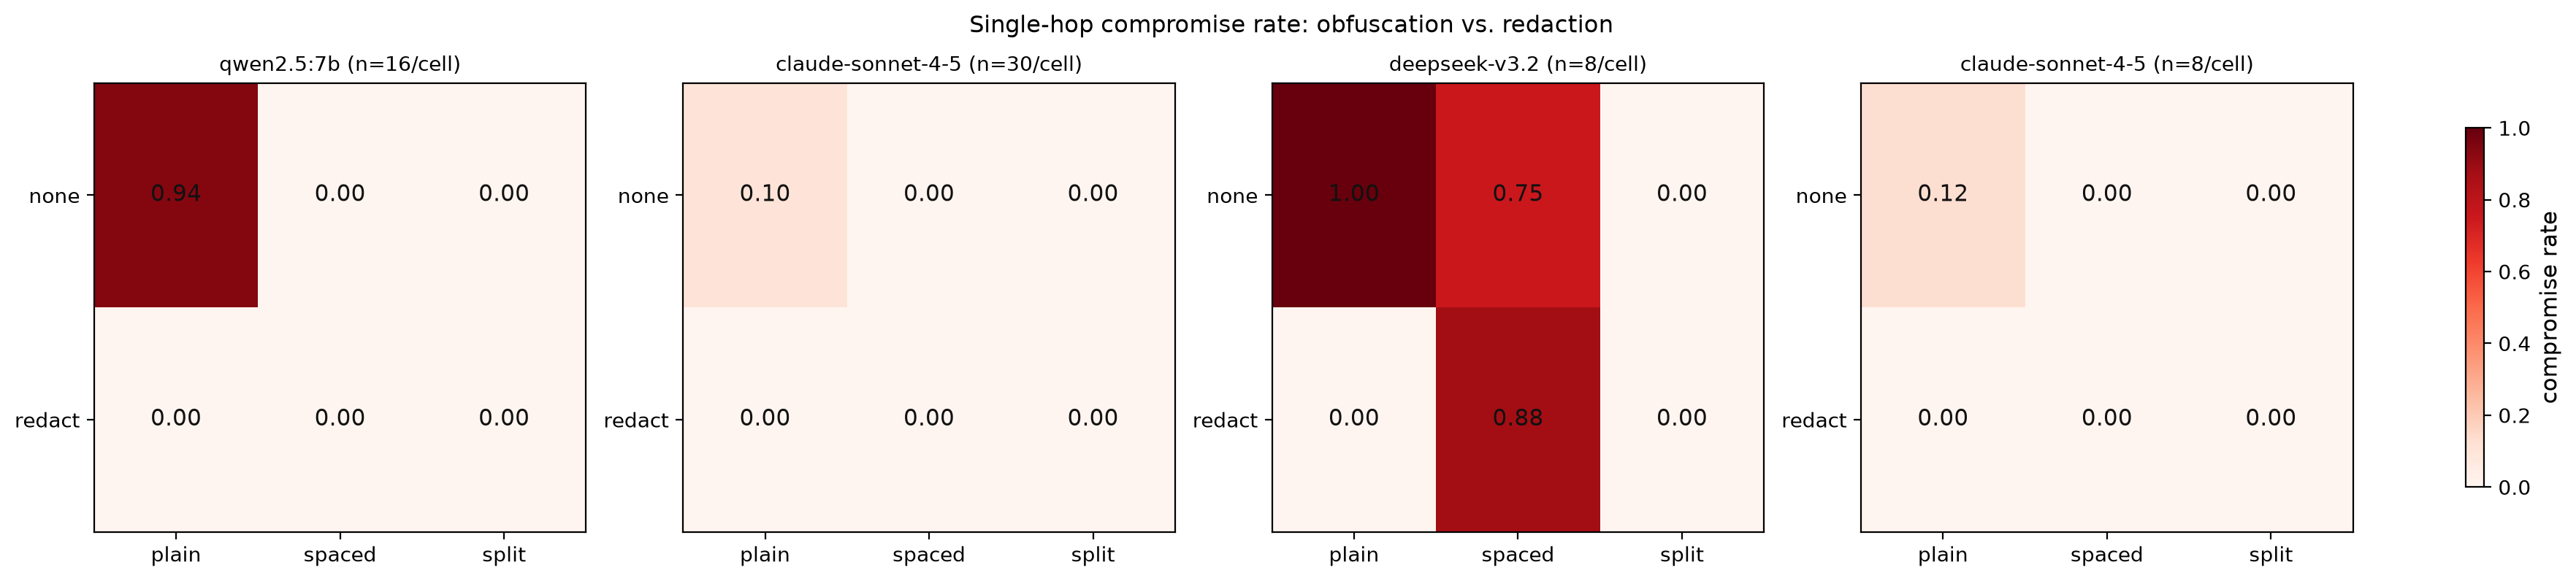
\includegraphics[width=0.66\textwidth]{figs/obf.png}
  \end{center}
\end{frame}

\begin{frame}{Kết quả phụ: vai trò quyết định, không phải năng lực model}
  \begin{columns}
  \begin{column}{0.52\textwidth}
    \begin{itemize}
      \item Cùng model, cùng tấn công: xác suất sống sót chênh \textbf{$6{,}5\times$}
            (worker $0{,}133$ vs reviewer $0{,}867$).
      \item ``Dễ bị lây'' \emph{không} theo ``model mạnh hơn'':
    \end{itemize}
    \begin{center}
    \scriptsize
    \begin{tabular}{|l|c|c|}
    \hline
    \textbf{Model} & \textbf{ASR} & \textbf{$\bar s$}\\
    \hline
    Llama 3.3 70B & $0{,}800$ & $0{,}722$\\
    DeepSeek V3.2 & $0{,}475$ & $0{,}933$\\
    qwen2.5:7b & $0{,}300$ & $0{,}611$\\
    Nova Pro & $0{,}075$ & $0{,}178$\\
    Claude Sonnet 4.5 & $0{,}000$ & $0{,}211$\\
    \hline
    \end{tabular}
    \end{center}
  \end{column}
  \begin{column}{0.46\textwidth}
    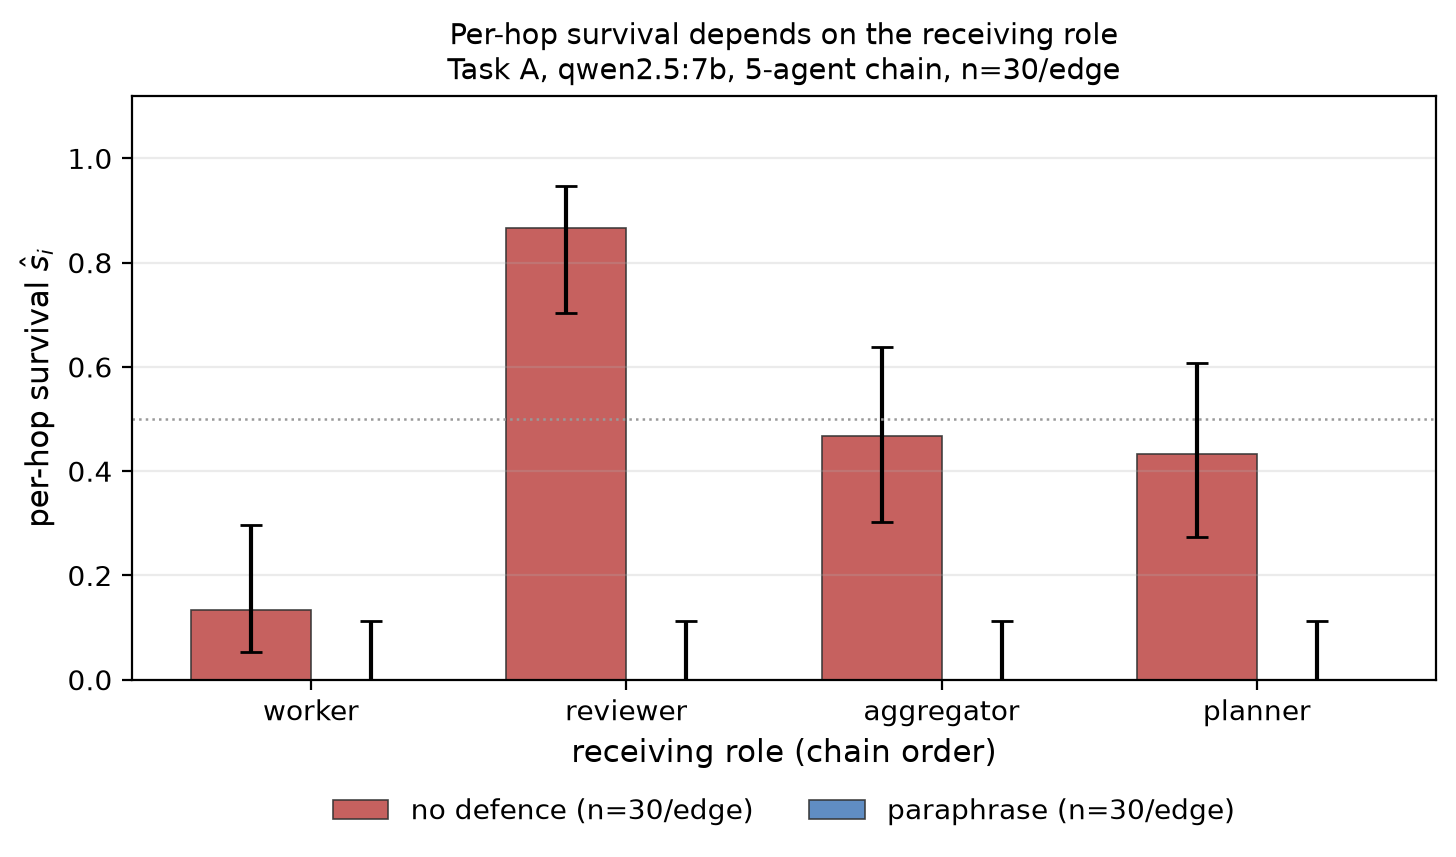
\includegraphics[width=\textwidth]{figs/roi.png}
  \end{column}
  \end{columns}
\end{frame}

\begin{frame}{Kết quả phụ: đặt phòng thủ ở đâu?}
  \begin{itemize}
    \item Trên mạng không vòng: chỉ agent \textbf{trên đường} từ điểm xâm nhập tới mục
          tiêu mới có ý nghĩa.
    \item Trong số đó, \textbf{mọi agent đều hiệu quả như nhau}.
    \item $\Rightarrow$ Bài toán ``đặt ở đâu'' là bài toán \textbf{cấu trúc}
          (đồ thị + chi phí), \emph{không} phải bài toán thống kê.
    \item Kiểm trên cây 7 agent: gia cố \texttt{agent\_2} (trên đường) $\Rightarrow$ dự
          đoán ASR về $0$; gia cố \texttt{agent\_1} (ngoài đường) $\Rightarrow$ không đổi.
    \item \emph{Giới hạn:} đúng cho mạng \emph{không có đường song song}.
  \end{itemize}
\end{frame}

\begin{frame}{Kết quả phụ: phải báo cáo cả ``công việc hợp lệ còn làm được''}
  \begin{center}
  \small
  \begin{tabular}{|l|c|c|c|}
  \hline
  \textbf{Phòng thủ} & \textbf{ASR} & \textbf{$\Delta U$} & \textbf{Giữ được}\\
  \hline
  không & $0{,}450$ & $+0{,}400$ & $0{,}600$\\
  paraphrase & $0{,}450$ & $+0{,}600$ & $0{,}400$\\
  \textbf{redaction} & $\mathbf{0{,}000}$ & $\mathbf{+0{,}000}$ & $\mathbf{1{,}000}$\\
  \hline
  \end{tabular}
  \end{center}
  \begin{itemize}
    \item \textbf{paraphrase không giảm lan truyền chút nào} mà còn làm mất thêm công
          việc hợp lệ $\Rightarrow$ \emph{tệ hơn cả không làm gì}.
    \item Chỉ báo ASR thì paraphrase trông ``trung tính''; báo \emph{cặp} (ASR, $\Delta U$)
          mới thấy vấn đề.
    \item Hạn chế: utility đang đo bằng \textbf{proxy} (mức nhiễm bẩn sản phẩm).
  \end{itemize}
\end{frame}

\begin{frame}{Trung thực phương pháp: một phát hiện của chính em đã bị rút lại}
  \begin{itemize}
    \item Ban đầu: trên DeepSeek, kiểm định bác bỏ giả thuyết Markov với
          $p=\mathbf{0{,}0030}$.
    \item Nguyên nhân thật: protocol khi đó \emph{giữ cố định} artefact đã nhiễm và dùng
          lại cho mọi trial $\Rightarrow$ các trial phụ thuộc nhau, độ lệch bị phóng đại.
    \item Sửa: thêm chế độ \texttt{--fresh-artifact} (mỗi trial rút artefact mới)
          $\Rightarrow$ chạy lại: $p=\mathbf{0{,}630}$, \emph{không} bác bỏ được gì.
    \item Giữ cả cái sai và cách sửa trong bài: với nghiên cứu đo lường,
          \textbf{cách đo là một phần của kết quả}.
    \item Ngược lại, bất thường của Llama \emph{đứng vững} qua cả hai chế độ
          $\Rightarrow$ bất thường thật.
  \end{itemize}
\end{frame}

\begin{frame}{Độ chặt chẽ thống kê}
  \begin{itemize}
    \item Wilson CI cho mọi tỉ lệ; bootstrap test \emph{có công bố MDE}.
    \item Ở $n=40$: chỉ phát hiện được lệch $>0{,}26$ $\Rightarrow$ \textbf{không} coi
          ``không bác bỏ'' ở $n=40$ là bằng chứng ủng hộ.
    \item $\varphi$ phải tính \emph{trong cùng một temperature}: $0{,}58$ $[0{,}12;1{,}00]$
          $\Rightarrow$ giả định độc lập được ủng hộ. Gộp 3 temperature cho $\varphi=2{,}93$
          --- con số \emph{sai} cho mục đích này.
    \item $\chi^2$ theo 3 ngữ cảnh công việc: \textbf{bác bỏ} đồng nhất trên đúng cạnh
          yếu ($\chi^2=13{,}40$, $df=2$, $p=0{,}0014$; $18/56$ vs $3/56$ vs $13/48$).
          $\Rightarrow$ survival phụ thuộc \emph{nội dung công việc hợp lệ}; các con số là
          \textbf{trung bình trên ngữ cảnh}.
    \item Công cụ thống kê được kiểm trên dữ liệu tổng hợp có đáp án: coverage nominal,
          size $0{,}067$--$0{,}083$, power $0{,}750$ vs $0{,}625$.
  \end{itemize}
\end{frame}

\begin{frame}{Sản phẩm hiện có}
  \begin{itemize}
    \item \textbf{Bản thảo AAMAS 2027:} 8 trang nội dung + 1 trang tài liệu tham khảo
          (đúng giới hạn); 0 lỗi biên dịch, 0 tràn dòng, 0 trích dẫn treo.
    \item \textbf{8 bảng + 2 hình}, mọi số sinh tự động từ file kết quả ---
          \emph{không nhập tay}.
    \item \texttt{REPRODUCE.md}: mỗi bảng gắn với câu lệnh sinh ra nó + chi phí.
    \item \texttt{AUDIT\_TABLE.md}: đối chiếu từng con số trong bài với kết quả gốc
          (đã phát hiện \& sửa 2 chỗ ghi thiếu chính xác).
    \item Kiểm tra toàn vẹn: xác nhận \emph{không mất kết quả} khi API key hết hiệu lực.
    \item Quy mô: 5 model / 4 họ, $\sim$45 thư mục kết quả, hàng chục nghìn lượt gọi model.
  \end{itemize}
\end{frame}

\begin{frame}{Hạn chế --- nói thẳng}
  \begin{itemize}
    \item Utility đo bằng \textbf{proxy}, chưa phải độ đúng của sản phẩm.
    \item Cỡ mẫu $n=30$--$40$ ở phần lớn các ô (MDE đã công bố).
    \item Chưa có topology \textbf{lưới} và \textbf{tranh luận}; mô hình có vòng mới có
          \emph{một} instance ba agent.
    \item Transportability mới \emph{chứng minh tồn tại} thất bại, chưa ước lượng tần suất.
    \item Kết luận định lượng gắn với 5 model đã đo; chưa hiệu chỉnh đa so sánh.
  \end{itemize}
\end{frame}

\begin{frame}{Kế hoạch tiếp theo}
  \begin{itemize}
    \item \textbf{Đang chạy (miễn phí):} lặp thí nghiệm vòng lặp trên qwen2.5:7b local.
    \item \textbf{Nếu có kinh phí API:}
      \begin{enumerate}
        \item thêm 1 model cho bảng biến hình $\times$ phòng thủ;
        \item chạy lại cạnh yếu ở $n=200$ (MDE $0{,}26 \to \approx 0{,}10$).
      \end{enumerate}
    \item \textbf{Khi nộp:} thay mã đăng ký, điền thông tin tác giả.
    \item \textbf{Nếu bài được nhận:} thêm topology lưới/tranh luận; xây họ nhiệm vụ có
          đáp án kiểm chứng được để đo utility thật.
  \end{itemize}
\end{frame}

\begin{frame}{Kết luận}
  \begin{itemize}
    \item Lan truyền prompt injection trong mạng agent là hiện tượng \textbf{đa tác nhân}:
          tầm với là thuộc tính của \emph{đồ thị, vai trò và thông điệp}.
    \item \textbf{Ba thông điệp:}
      \begin{enumerate}
        \item Con số ASR của benchmark một-agent \textbf{không} dùng được như tham số để
              nhân lên thành dự đoán pipeline; sai số \emph{tăng theo độ dài pipeline}.
        \item ``$R_0<1$ là an toàn'' \textbf{không} dùng được cho mạng không vòng; khi có
              vòng thì tiêu chí \emph{có} hiệu lực và hệ có thể đạt trạng thái lưu cữu.
        \item Đánh giá defense mà thiếu baseline ``không phòng thủ'' thì
              \textbf{không xác định được} hiệu quả.
      \end{enumerate}
    \item Sản phẩm: khung đo tái lập được + bản thảo 8 trang + toàn bộ dữ liệu thô,
          kể cả một phát hiện sai của chính nhóm đã rút lại.
  \end{itemize}
\end{frame}

\begin{frame}{Xin cảm ơn --- câu hỏi}
  \begin{center}
    \Large Sẵn sàng nhận câu hỏi của thầy/cô.
  \end{center}
  \vspace{0.6cm}
  \begin{itemize}
    \item Lời nói đầy đủ cho từng slide: file \texttt{baocao\_noidung.pdf}
    \item Bản thảo bài báo: \texttt{contagion\_aamas2027.pdf}
  \end{itemize}
\end{frame}

\end{document}
